\documentclass[10pt,a4paper,landscape]{article}
\usepackage[utf8]{inputenc}
\usepackage[T1]{fontenc}
\usepackage{amsmath}
\usepackage{amsfonts}
\usepackage{amssymb}
\usepackage{graphicx}
\usepackage{lscape}
\usepackage{multirow}
\usepackage{array}
\usepackage{lmodern}
\usepackage[OT1]{fontenc}
\usepackage[utf8]{inputenc}
\usepackage[none]{hyphenat}
\usepackage{fancyhdr}
\usepackage{eso-pic, graphicx}
\usepackage{geometry}[left=0.5cm, bottom=0.5cm, right=0.5, top=0.5cm]
\usepackage[french]{babel}


\graphicspath{ {\VAR{image_path}} }
\newcommand\BackgroundPic{
\put(-4,0){
\parbox[b][\paperheight]{\paperwidth}{
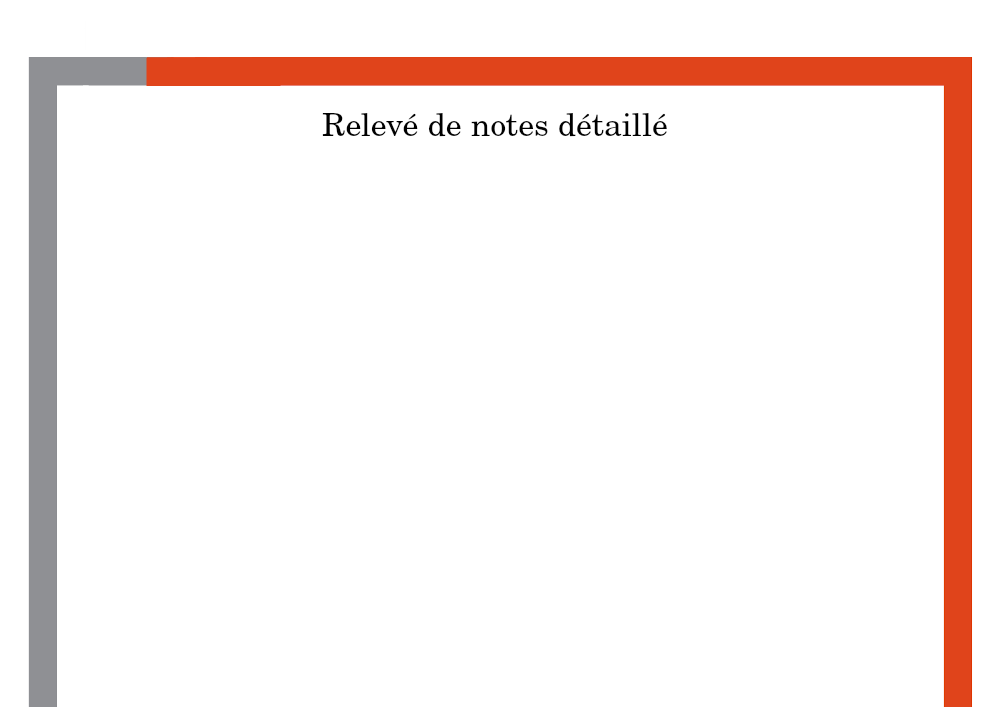
\includegraphics[width=\paperwidth,height=\paperheight]{CharteGraphiquePresentationPageDeGarde}
}}}




\begin{document}  
 

\begin{center}
\huge
Récapitulatif du semestre \VAR{semestre.libelle} - \VAR{annee}
\end{center}

%faire une boucle qui compte et additionne pour chaque ue , le nombre de matiere , recuperer la valeur total de matiere et y ajouter 2
%la valeur ainsi recuperer , on fait une boucle pour creer le begin tabular et  la valeur correspond au nombre de |c|


\vspace{0.5cm}
\hspace{-3cm}
\begin{tabular}{\VAR{partie_1['colonnes']}}
%ensuite pour le cline on par de 3 jusqua cette valeur recuperer
\cline{3-\VAR{partie_1['nbre_colonnes']}}
%ensuite ici on met la premierer ligne (\multicolumn{2}{c|}{} &) et  on fait une boucle pour recuperer les ue , pour chaque ue , on recupere une valeur correspondante au nombre de matiere que comprend l'ue et on la met ensuite dabs le multicolumn , et dans les crochet , de fin , on ajoute le libelle de l'ue
\multicolumn{2}{c|}{} & 
\BLOCK{for ue in range(partie_1['nbre_ues'] -1)}
  \multicolumn{\VAR{partie_1['lignes'][0]['ues'][ue]['nbre_matieres']}}{p{3cm}|}{\centering \VAR{partie_1['lignes'][0]['ues'][ue]['ue'].libelle}} & 
\BLOCK{endfor}
\multicolumn{\VAR{partie_1['lignes'][0]['ues'][partie_1['nbre_ues'] -1]['nbre_matieres']}}{p{3cm}|}{\centering \VAR{partie_1['lignes'][0]['ues'][partie_1['nbre_ues'] -1]['ue'].libelle}}\\ 

% on vient ensuite ici apres le hline , on met (Prénom & Nom & ) et on boucle ensuite pour recuperer dans l'odre des ue , les libellle de chacune des matieres des ue et on les met dans les crochet avec la proprieter centring
\hline 
\centering Nom & \centering Prenom & 
\BLOCK{for ue in range(partie_1['nbre_ues'] -1)}
  \BLOCK{for matiere in partie_1['lignes'][0]['ues'][ue]['matieres_ue']}
    \rotatebox{90}{\parbox[c]{2.5cm}{\centering \VAR{matiere['matiere'].abbreviation} }}  & 
  \BLOCK{endfor} 
\rotatebox{90}{\parbox[c]{2.5cm}{\centering \textbf{UE} }} & \rotatebox{90}{\parbox[c]{2.5cm}{\centering \textbf{Crédits} }} &
\BLOCK{endfor} 

\BLOCK{for matiere in partie_1['lignes'][0]['ues'][partie_1['nbre_ues'] -1]['matieres_ue']}
\rotatebox{90}{\parbox[c]{2.5cm}{\centering \VAR{matiere['matiere'].abbreviation} }}  & 
\BLOCK{endfor} 
\rotatebox{90}{\parbox[c]{2.5cm}{\centering \textbf{UE} }} & \rotatebox{90}{\parbox[c]{2.5cm}{\centering \textbf{Crédits} }}  \\

% ensuite ici on ferme en mettant un intervale de la valeur recuperer , qui par de cet valeur a cette valeur dans l'element cline
\cline{\VAR{partie_1['nbre_colonnes']}-\VAR{partie_1['nbre_colonnes']}}

%ici on fait une boucle pour compter le nombre d'eleve et pour chaque eleve , on genere une ligne de l'element hline qui prend le prenom , le nom , et la moyenne pour chaque matiere dans l'ordre 
\hline 

\BLOCK{for i in range(partie_1['nbre_lignes'])}

  \VAR{partie_1['lignes'][i]['etudiant'].nom} & \VAR{partie_1['lignes'][i]['etudiant'].prenom} & 

  \BLOCK{for ue in range(partie_1['nbre_ues'] -1)}

    \BLOCK{for matiere in partie_1['lignes'][i]['ues'][ue]['matieres_ue']}
      \VAR{matiere['moyenne_matiere']}  & 
    \BLOCK{endfor} 

    \textbf{\VAR{partie_1['lignes'][i]['ues'][ue]['moyenne']}}  & 

    \BLOCK{if partie_1['lignes'][i]['ues'][ue]['a_valide']}
      \textbf{\VAR{partie_1['lignes'][i]['ues'][ue]['ue'].nbreCredits}}
    \BLOCK{else}
      \textbf{0}
    \BLOCK{endif}
    &
  \BLOCK{endfor}

  \BLOCK{for matiere in partie_1['lignes'][i]['ues'][partie_1['nbre_ues'] -1]['matieres_ue']}
    \VAR{matiere['moyenne_matiere']}  & 
  \BLOCK{endfor} 

  \textbf{\VAR{partie_1['lignes'][i]['ues'][partie_1['nbre_ues'] -1]['moyenne']}} & 
    \BLOCK{if partie_1['lignes'][i]['ues'][partie_1['nbre_ues'] -1]['a_valide']}
      \textbf{\VAR{partie_1['lignes'][i]['ues'][partie_1['nbre_ues'] -1]['ue'].nbreCredits}}
    \BLOCK{else}
      \textbf{0}
    \BLOCK{endif}
  \\

\hline
\BLOCK{endfor}



\end{tabular} 



\newpage

\BLOCK{if partie_2}

\hspace{-3cm}
\begin{tabular}{\VAR{partie_2['colonnes']}}
%ensuite pour le cline on par de 3 jusqua cette valeur recuperer
\cline{3-\VAR{partie_2['nbre_colonnes']}}
%ensuite ici on met la premierer ligne (\multicolumn{2}{c|}{} &) et  on fait une boucle pour recuperer les ue , pour chaque ue , on recupere une valeur correspondante au nombre de matiere que comprend l'ue et on la met ensuite dabs le multicolumn , et dans les crochet , de fin , on ajoute le libelle de l'ue
\multicolumn{2}{c|}{} & 
\BLOCK{for ue in range(partie_2['nbre_ues'] -1)}
  \multicolumn{\VAR{partie_2['lignes'][0]['ues'][ue]['nbre_matieres']}}{p{3cm}|}{\centering \VAR{partie_2['lignes'][0]['ues'][ue]['ue'].libelle}} & 
\BLOCK{endfor}
\multicolumn{\VAR{partie_2['lignes'][0]['ues'][partie_2['nbre_ues'] -1]['nbre_matieres']}}{p{3cm}|}{\centering \VAR{partie_2['lignes'][0]['ues'][partie_2['nbre_ues'] -1]['ue'].libelle}} & Total crédits\\ 

% on vient ensuite ici apres le hline , on met (Prénom & Nom & ) et on boucle ensuite pour recuperer dans l'odre des ue , les libellle de chacune des matieres des ue et on les met dans les crochet avec la proprieter centring
\hline 
Nom & Prenom & 
\BLOCK{for ue in range(partie_2['nbre_ues'] -1)}
  \BLOCK{for matiere in partie_2['lignes'][0]['ues'][ue]['matieres_ue']}
    \rotatebox{90}{\parbox[c]{2.5cm}{\centering \VAR{matiere['matiere'].abbreviation} }}  & 
  \BLOCK{endfor} 
\rotatebox{90}{\parbox[c]{2.5cm}{\centering \textbf{UE} }} & \rotatebox{90}{\parbox[c]{2.5cm}{\centering \textbf{Crédits} }} &
\BLOCK{endfor} 

\BLOCK{for matiere in partie_2['lignes'][0]['ues'][partie_2['nbre_ues'] -1]['matieres_ue']}
\rotatebox{90}{\parbox[c]{2.5cm}{\centering \VAR{matiere['matiere'].abbreviation} }}  & 
\BLOCK{endfor} 
\rotatebox{90}{\parbox[c]{2.5cm}{\centering \textbf{UE} }} & \rotatebox{90}{\parbox[c]{2.5cm}{\centering \textbf{Crédits} }} &  \\

% ensuite ici on ferme en mettant un intervale de la valeur recuperer , qui par de cet valeur a cette valeur dans l'element cline
\cline{\VAR{partie_2['nbre_colonnes']}-\VAR{partie_2['nbre_colonnes']}}

%ici on fait une boucle pour compter le nombre d'eleve et pour chaque eleve , on genere une ligne de l'element hline qui prend le prenom , le nom , et la moyenne pour chaque matiere dans l'ordre 
\hline 

\BLOCK{for i in range(partie_2['nbre_lignes'])}

  \VAR{partie_2['lignes'][i]['etudiant'].nom} & \VAR{partie_2['lignes'][i]['etudiant'].prenom} & 

  \BLOCK{for ue in range(partie_2['nbre_ues'] -1)}

    \BLOCK{for matiere in partie_2['lignes'][i]['ues'][ue]['matieres_ue']}
      \VAR{matiere['moyenne_matiere']}  & 
    \BLOCK{endfor} 

    \textbf{\VAR{partie_2['lignes'][i]['ues'][ue]['moyenne']}}  & 

    \BLOCK{if partie_2['lignes'][i]['ues'][ue]['a_valide']}
      \textbf{\VAR{partie_2['lignes'][i]['ues'][ue]['ue'].nbreCredits}}
    \BLOCK{else}
      \textbf{0}
    \BLOCK{endif}
    &
  \BLOCK{endfor}

  \BLOCK{for matiere in partie_2['lignes'][i]['ues'][partie_2['nbre_ues'] -1]['matieres_ue']}
    \VAR{matiere['moyenne_matiere']}  & 
  \BLOCK{endfor} 

  \textbf{\VAR{partie_2['lignes'][i]['ues'][partie_2['nbre_ues'] -1]['moyenne']}} & 
    \BLOCK{if partie_2['lignes'][i]['ues'][partie_2['nbre_ues'] -1]['a_valide']}
      \textbf{\VAR{partie_2['lignes'][i]['ues'][partie_2['nbre_ues'] -1]['ue'].nbreCredits}}
    \BLOCK{else}
      \textbf{0}
    \BLOCK{endif}
    &
    \textbf{\VAR{partie_2['lignes'][i]['ues'][partie_2['nbre_ues'] -1]['credits_semestre']}}
  \\

\hline
\BLOCK{endfor}



\end{tabular} 


\BLOCK{endif}



% un dictionnaire qui qui a le nombre de matiere par ue et le libelle de cette ue
% un tableau des libelle de chacune des matiere
% une donnee longueur tableau qui est le nombre de matiere total pour les ue + 2 
% j'ai besoin d'un dictionnaire qui pour chaque etudiant , regroupe son prenom , son nom et chacune des moyennes de chacune de ses matieres




\end{document}